\chapter{Modelling of electrokinetic flow}
kcl ref to appendix...
\begin{table}
  \caption{Physical parameters of a KCl ion solution that is modelled
    in this chapter. Parameters are from \cite{dongquing-ren-book}. }
\begin{center}
    \begin{tabular}{ | r | l |}
    \hline
    Relative permittivity, $\ep_r$ & 80\\
    Mean ionic conentration, $\cnil$ & $10^{-4}$ mol/m$^3$\\
    Conductivity, $\sigma_c$ & 1.5 mS/m\\
    Temperature, T & 293 K\\
    kinematic viscosity, $\nu$ & 1.0 $\mu$m$^2$/s\\
    Diffusion coefficient, $D_+ = D_{-}$ & $ 10^{-10}$ m$^2$/s\\
    \hline
    \end{tabular}
\end{center}    
\label{tab:res:param}
\end{table}

\section{Charge concentration and potential in 1D system}
section in the channel, + debye-huckel comparision

\begin{figure}
\begin{center}
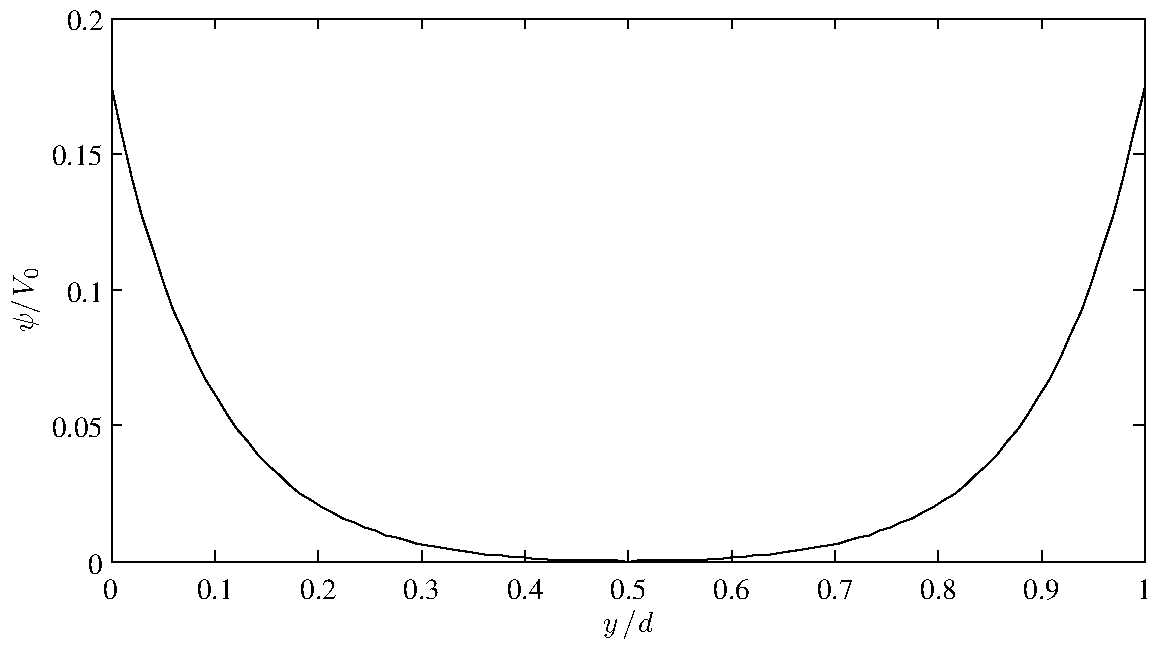
\includegraphics[width=0.9\textwidth]{fig/potential_1d.pdf}
\end{center}
\caption{Computed electric potential across a channel of width $d = 10
  \mu$m. The solution in the channel is a KCl solution defined by
  parameters in table \ref{tab:res:param}. The channel walls are
  negatively charged. Note that $\Vnil$ is negative.}
\label{fig:res:pot_1d}
\end{figure}

\begin{figure}
\begin{center}
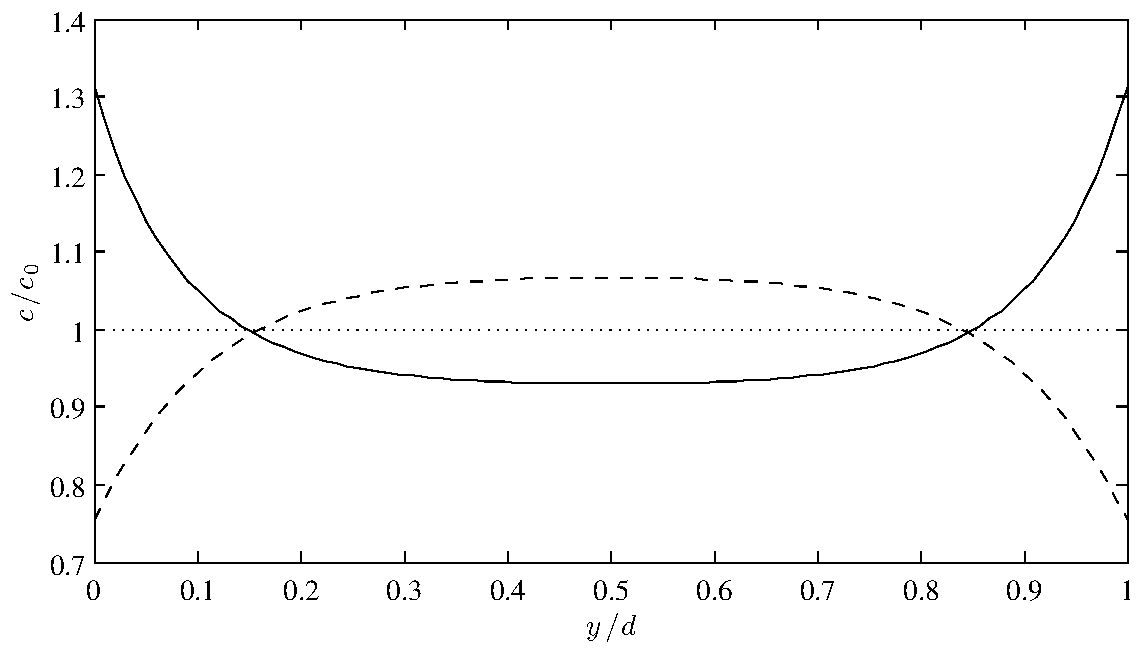
\includegraphics[width=0.9\textwidth]{fig/charge_1d.pdf}
\end{center}
\caption{Computed positive (solid) and negative (dashed) charge
  distribution across a channel of width $d = 10 \mu$m. The solution
  in the channel is a KCl solution defined by parameters in table
  \ref{tab:res:param}. The channel walls are negatively charged.}
\label{fig:res:c_1d}
\end{figure}

\subsection{Nernst-Planck vs. Poisson-Boltzmann}

\section{Electroviscous effect}

\section{Electroosmotic flow}
NP + PB differences?
\section{Flow in channel with heterogeneously charged walls}

\section{Flow in array of charged squares}
